\paragraph{Prospect}
In order to extend this project and to improve the accuracy various approaches can be considered in future research. 

One of the first problems regarding the missing values of budget and revenue could be targeted with additional information sources. Where this project relies on the external sources from \textit{IMDB } and \textit{the Numbers} also other sources can be taken into account. The more reliable information provieded, the easier the dataset can be expanded back to the original set of 45,000 entries.

\huge hier muss noch was zum wrapper hin?


\normalsize Including  more powerful features might be another possibility to increase the value of the dataset. In this project; members from the crew are limited to actors and directors of each movie. Improvement might be reached through adding more famous and know members as for example writers. Also the popularity of each movie could be taken into account as it is already provided inside the data set. 
In order to gain more insights of the movie's topic a sentiment analysis could be performed on the description of each movie. By running a sentiment analysis most interesting topics could be calculated, and correlated with the popular vote of each movie. Further reasearch should therefore focus on bringing all the necessary information together and make it more valuable for the data mining process.

%\begin{itemize}
%	\item find other data sources for revenue / budget values to expand the data set with additional movies
%	\item try other feature selection methods (backward wrapper, filter)
%	\item add additional features
%	\begin{itemize}
%		\item popularity of the actors / crew
%		\item add additional crew members (e.g. writer)
%		\item extract key phrases from the synopsis of the movie
%	\end{itemize}
%\end{itemize}
%
\label{cha:prospect}
\begin{figure}[h]
	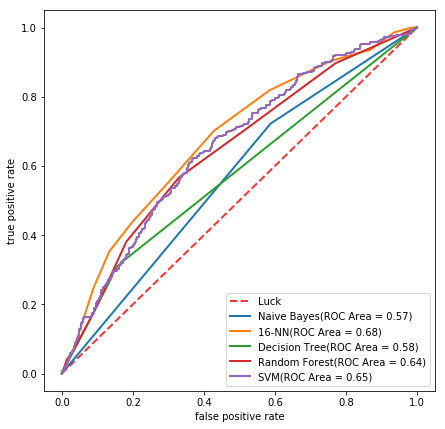
\includegraphics[width=\textwidth]{images/roc.png}
	\caption{Macro average ROC Curves for all classifiers}
	\label{img:roc}
\end{figure}
\FloatBarrier